\section{Implementation}\label{sec:Implementation}
% ! Nuclear option: Linux dual-boot and screenshot as you go on it.

\subsection{Software requirements}
% Talk about Visual Studio Code.
% Talk about Python and the modules themselves. Did any of them have logins?
% Talk about OpenAI setup.
The project was developed using Visual Studio Code as a development environment and Python as the programming language.
Both of these are available freely with no limitation for academic use.

\para Many Python modules were used, with the UV package manager \autocite{astralUv} being used for their installation 
due to its own high speed and ease of use. The version of Python used was 3.9.2 to ensure compatibility with the wide variety 
of modules used, which are detailed in Table \ref{tab:PythonModules}.

\begin{longtable}{ | p{0.25\textwidth} | p{0.7\textwidth} | }
    \hline
    \cellcolor{blue!25} Module(s) & \cellcolor{blue!25} Purpose \\
    \hline
    langchain & The framework used to handle LLM interactions, as well as embedding documents and user queries. \\
    \hline
    langchain-community & Provides additional helper classes and functions to assist development. \\
    \hline 
    langchain-openai \newline 
    openai & Provides the functions used to interact with OpenAI models such as gpt-4o-mini and text-embedding-3-small in LangChain. \\
    \hline 
    langgraph & Used to create a directed sequence of events for the chatbot to execute. A major part of the backend, further described 
    in Section \ref{sec:ChatbotBackend}. \\
    \hline
    pdfminer-six \newline 
    pypdf & Dependencies of LangChain for PDF reading. \\
    \hline 
    Streamlit & Used as the frontend of the chatbot and also stores the conversation in memory. Described further in Section 
    \ref{sec:ChatbotFrontend}. \\
    \hline
    \caption{The Python modules used in the project's development.}\label{tab:PythonModules}
\end{longtable}



\subsection{Data storage}
% Talk about getting University policies from their site. Provide URL or Harvard reference it?
% Talk about your own added info document you made in LaTeX.
% Talk about embedding the policies.
The backbone of this project is the BCU-related data that the chatbot will pull from when queried.
The vast majority of this data was sourced from the official Birmingham City University website \autocite{bcuPoliciesProcedures},
where individual policies are stored as PDF files for public download without any access limitations or restrictions.
An observation made through an analysis of many of the policies was that none of them explicitly state key information about the university,
such as campus building locations or information about its student union. Therefore, an additional document of my own creation with \LaTeX
was included amongst the downloaded data. This document contained key information about BCU itself, with information on campus addresses 
and miscellaneous helpful information for students.

\para With all documents downloaded or created, the next stage would be to incorporate them in a format an LLM can interpret. This introduces 
LangChain, a popular framework for LLM app development \autocite{langchain_introduction_nodate}, which provides helper classes to directly read 
PDF files from a directory and split the text data within into smaller chunks, as seen in Figure \ref{fig:LangChainDocumentLoader}.

\begin{figure}[H]
    \centering
    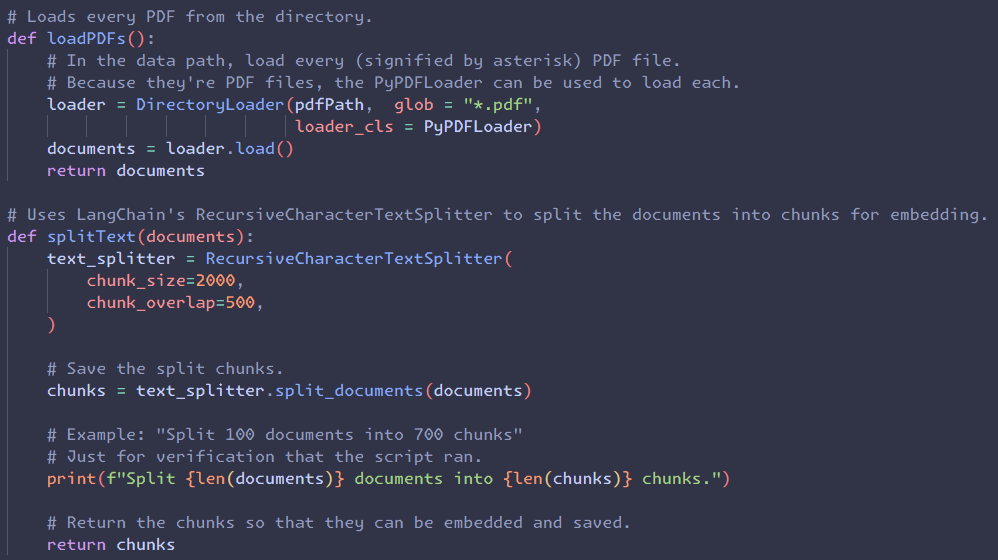
\includegraphics[width=0.8\textwidth]{Artefact/DocumentLoader.png}
    \caption{Code used to load all PDFs from the Policies directory and split them into chunks. \label{fig:LangChainDocumentLoader}}
\end{figure}

\noindent Once these chunks have been created, they must then be embedded as vectors, which will allow an LLM to interpret them. These 
vectors were then stored in a Facebook AI Similarity Search (FAISS) database as researched in Section \ref{sec:LitReviewRAG}, which 
ensured that the policies only needed to be embedded once rather than every time the chatbot was run.

\begin{figure}[H]
    \centering
    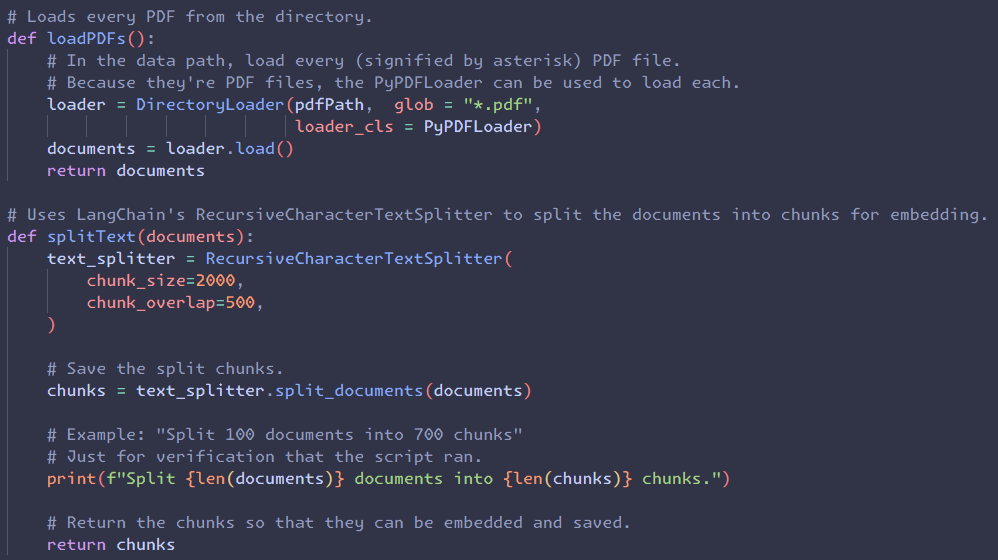
\includegraphics[width=0.8\textwidth]{Artefact/DocumentLoader.png}
    \caption{Code used to embed and store the chunks into a FAISS DB. \label{fig:LangChainStoreFAISS}}
\end{figure}

% ! Screenshot of this running if possible.



\subsection{Chatbot backend}\label{sec:ChatbotBackend}
% Talk about LangChain and LangGraph.


\subsection{Accessing the chatbot}\label{sec:ChatbotFrontend}
% Talk about Streamlit.
% Show example conversations here or perhaps make another section for them.

